\begin{figure}
	\centering
	\pgfplotsset{every axis legend/.append style={
		at={(1.05,0.5)},
		anchor=west}}
	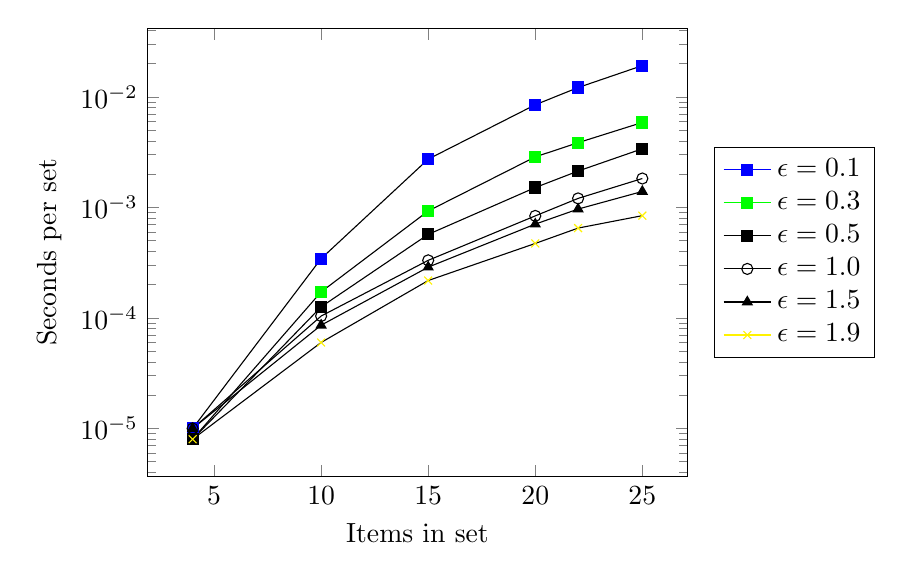
\begin{tikzpicture}
		\begin{semilogyaxis}[
			xlabel=Items in set,
			ylabel=Seconds per set,
			scatter/classes={
				fptas1={mark=square*,blue},
				% fptas2={mark=square*,red},
				fptas3={mark=square*,green},
				% fptas4={mark=square*,yellow},
				fptas5={mark=square*,black},
				% fptas6={mark=o,blue},
				% fptas7={mark=o,red},
				% fptas8={mark=o,green},
				% fptas9={mark=o,yellow},
				fptas10={mark=o,black},
				% fptas11={mark=triangle*,blue},
				% fptas12={mark=triangle*,red},
				% fptas13={mark=triangle*,green},
				% fptas14={mark=triangle*,yellow},
				fptas15={mark=triangle*,black},
				% fptas16={mark=x,blue},
				% fptas17={mark=x,red},
				% fptas18={mark=x,green},
				fptas19={mark=x,yellow}
				}
            ]
            
\addplot[scatter,scatter src=explicit symbolic]table[meta=label] {
x y label
4 .000010 fptas1
10 .000344 fptas1
15 .002732 fptas1
20 .008480 fptas1
22 .012136 fptas1
25 .019182 fptas1
};
\addplot[scatter,scatter src=explicit symbolic]table[meta=label] {
x y label
4 .000008 fptas3
10 .000172 fptas3
15 .000928 fptas3
20 .002864 fptas3
22 .003850 fptas3
25 .005866 fptas3
};
\addplot[scatter,scatter src=explicit symbolic]table[meta=label] {
x y label
4 .000008 fptas5
10 .000126 fptas5
15 .000570 fptas5
20 .001512 fptas5
22 .002132 fptas5
25 .003392 fptas5
};
\addplot[scatter,scatter src=explicit symbolic]table[meta=label] {
x y label
4 .000010 fptas10
10 .000104 fptas10
15 .000332 fptas10
20 .000838 fptas10
22 .001206 fptas10
25 .001826 fptas10
};
\addplot[scatter,scatter src=explicit symbolic]table[meta=label] {
x y label
4 .000010 fptas15
10 .000086 fptas15
15 .000288 fptas15
20 .000706 fptas15
22 .000966 fptas15
25 .001394 fptas15
};
\addplot[scatter,scatter src=explicit symbolic]table[meta=label] {
x y label
4 .000008 fptas19
10 .000060 fptas19
15 .000218 fptas19
20 .000472 fptas19
22 .000650 fptas19
25 .000842 fptas19
};

			\addlegendentry{$\epsilon = 0.1$}
			\addlegendentry{$\epsilon = 0.3$}
			\addlegendentry{$\epsilon = 0.5$}
			\addlegendentry{$\epsilon = 1.0$}
			\addlegendentry{$\epsilon = 1.5$}
			\addlegendentry{$\epsilon = 1.9$}
		\end{semilogyaxis}
	\end{tikzpicture}
\caption{Time needed for maximal deviation}
\label{plot:fptasTime}
\end{figure}
